% Supplementary material for Mode-II, input at the end of main.tex
\section{Closure ladder}\label{supp:closure}
The held-out $R^2$ values behind \S\ref{sec:flow}, transcribed from the findings ledger.

\begin{figure}[h]
 \centering
 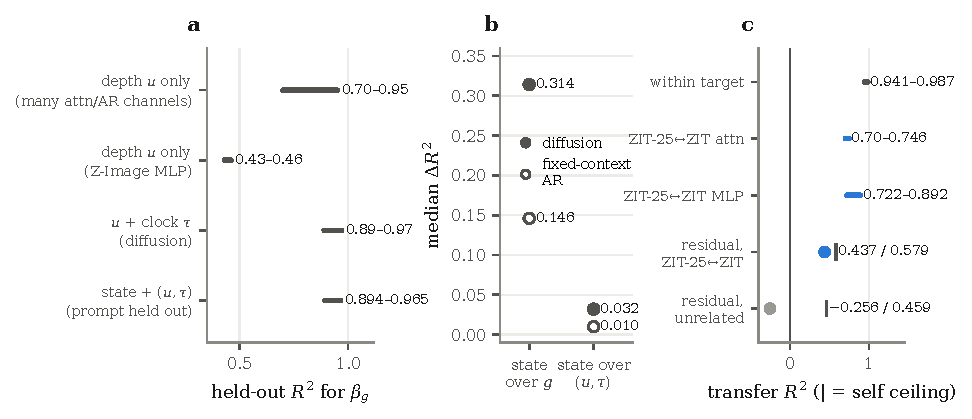
\includegraphics[width=\linewidth]{II-F4_closure_ladder}
 \caption{\textbf{Nonautonomous closure ladder.} Values are transcribed from the findings ledger. The ledger reports ranges and medians, not per-channel tables, so ranges are drawn as intervals. (a) Held-out $R^2$ for the layer-direction flow $\beta_g$: depth $u$ alone: 0.70--0.95 in many attention/AR channels, but only 0.43--0.46 in Z-Image MLP; $u$ plus the clock $\tau$: 0.89--0.97 in diffusion; local state plus coordinates with whole prompts held out: 0.894--0.965 (D01). (b) Median incremental $R^2$. The spectral state $[g,{\rm gap},H]$ adds $+0.314$ (diffusion) and $+0.146$ (fixed-context AR) over $g$ alone. Once a flexible learner has $(u,\tau)$, the full state adds only $+0.032$ (diffusion) and $+0.010$ (AR), or $+0.014$ overall. Under the frozen minimal-sufficiency rule, 7/12 channels need only $(u,\tau)$ and 5/12 need $g+u+\tau$ (D08/D09). This ladder is close to true by construction once the scaffold holds $96\%$ of the variance (\S\ref{sec:flow}); it describes how the measured manifold is parametrised, and the non-autonomy argument rests on the transfer results in (c) and Table~\ref{tab:transfer}. (c) Vector-field transfer: within target: 0.941--0.987; \TT{}$\leftrightarrow$ZIT (same Turbo weights): attention 0.700--0.746, MLP 0.722--0.892 (D03); residual after scaffold subtraction: \TT{}$\leftrightarrow$ZIT 0.437 against a self ceiling of 0.579, unrelated pairs $-0.256$ against $\approx0.459$ (D15). Transfer into Mochi and SD3.5 M/L is "approximately zero or negative" (D03). No value is tabulated for it, so it is not plotted. Together these support a model-specific nonautonomous family $\dot z=F_m^{(0)}(u,\tau)+R_m(z,u,\tau)$ and reject a universal autonomous $\beta(g)$ or a universal microscopic $F$ (register T5). Sources: ledger cards "Depth coordinate is a major explanatory variable" (script 15), "Cross-substrate CoS state\ldots{}" (script 11), D01, D03, D08/D09 and D15.}
 \label{fig:closure}
\end{figure}

\section{Intrinsic arc-length reparameterisation}\label{app:arclength}
Reparameterising each coarse curve by cumulative spectral arc length raises unrelated and cross-channel correlations by $+0.057$ on average, changes the comparison of \TT{} with ZIT (the same Turbo weights) by $-0.004$, and the preregistered paired test is not significant ($p\approx0.105$, D17). Arc length is therefore not a decisive universal progress variable.

\section{Legacy rebound and complex-mode study}\label{app:legacy}
Fitting $z(\ell+1)=Az(\ell)+b$ with $z=(g,-\gap,H)$ on the final rebound branch of SD3.5 Medium depth profiles gives a complex-conjugate pair with modulus below one at all three resolutions, retained in 500 of 500 generation-cluster bootstraps, median moduli $0.526$ ($512$), $0.501$ ($768$), $0.400$ ($1024$). These files were recorded with a hook that substitutes an exponential-moving-average attention path whenever it is registered, on a single prompt; in a matched CFG study the complex mode exists only in steps 0--9, and over all 100 steps CFG 1.0 has no complex pair. We report the study as a historical exploration with that instrument caveat, not as release evidence.

\section{Envelope trend ratios and coordinate collinearity}\label{supp:kappa}
\begin{table}[htbp]
\centering\small
\caption{Trend-dominance floor of Proposition~7 per pair (post hoc, Mode-I RC25). Layer-mean attention $g$ of the five archive campaigns on a common $\sigma$ grid; trend $T$ = the five-model mean envelope (descriptive: it contains both models of each pair). $\kappa=\operatorname{Var}(r)/(\alpha^2\operatorname{Var}T)$; floor $=(1-\sqrt{\kappa_a\kappa_b})/\sqrt{(1+\kappa_a)(1+\kappa_b)}$; observed: the envelope correlation. Values for $T$ linear in $\sigma$ are in \texttt{rc25\_kappa\_pairs.csv}.}
\label{tab:kappa}
\begin{tabular}{llcccc}
\toprule
Pair & Relation & $\kappa_a$ & $\kappa_b$ & Floor & Observed\\
\midrule
ZIT $\leftrightarrow$ Mochi & unrelated & 0.078 & 0.355 & 0.690 & 0.707\\
ZIT $\leftrightarrow$ SD3.5 M & unrelated & 0.078 & 0.156 & 0.797 & 0.969\\
ZIT $\leftrightarrow$ SD3.5 L & unrelated & 0.078 & 0.010 & 0.931 & 0.976\\
\TT{} $\leftrightarrow$ Mochi & unrelated & 0.042 & 0.355 & 0.739 & 0.923\\
\TT{} $\leftrightarrow$ SD3.5 M & unrelated & 0.042 & 0.156 & 0.837 & 0.846\\
\TT{} $\leftrightarrow$ SD3.5 L & unrelated & 0.042 & 0.010 & 0.954 & 0.960\\
Mochi $\leftrightarrow$ SD3.5 M & unrelated & 0.355 & 0.156 & 0.611 & 0.624\\
Mochi $\leftrightarrow$ SD3.5 L & unrelated & 0.355 & 0.010 & 0.803 & 0.808\\
SD3.5 M $\leftrightarrow$ SD3.5 L & same family & 0.156 & 0.010 & 0.888 & 0.958\\
\bottomrule
\end{tabular}
\end{table}

\begin{table}[htbp]
\centering\small
\caption{Spearman correlations between the coordinates over all (generation, state, layer) cells of each cube (post hoc, Mode-I RC31). The first seven rows are the archive cubes behind Remark~\ref{rem:dims} (its range, $0.93$--$0.97$ and $-0.79$ to $-0.20$); the rest are the Round 12--17 cubes.}
\label{tab:collin}
\begin{tabular}{llrccc}
\toprule
Cube & Hook & Cells & $\log g$, $H$ & $\log g$, $\log\gap$ & $H$, $\log\gap$\\
\midrule
ZIT & attn & 115{,}200 & 0.963 & $-$0.730 & $-$0.660\\
ZIT & MLP & 115{,}200 & 0.969 & $-$0.456 & $-$0.304\\
\TT{} & attn & 357{,}000 & 0.969 & $-$0.760 & $-$0.709\\
\TT{} & MLP & 357{,}000 & 0.972 & $-$0.513 & $-$0.384\\
Mochi & attn & 688{,}320 & 0.974 & $-$0.787 & $-$0.745\\
SD3.5 M & attn & 460{,}800 & 0.939 & $-$0.203 & $-$0.059\\
SD3.5 L & attn & 516{,}040 & 0.926 & $-$0.516 & $-$0.364\\
Z1 (Base) & attn & 359{,}250 & 0.969 & $-$0.780 & $-$0.724\\
Z1 (Base) & MLP & 358{,}500 & 0.952 & $-$0.527 & $-$0.333\\
Z3 (Turbo{,} Base settings) & attn & 90{,}000 & 0.956 & $-$0.698 & $-$0.612\\
Z3 (Turbo{,} Base settings) & MLP & 90{,}000 & 0.972 & $-$0.505 & $-$0.363\\
ACE-Step Base & attn & 72{,}000 & 0.962 & $-$0.297 & $-$0.250\\
ACE-Step Base & MLP & 72{,}000 & 0.960 & $-$0.337 & $-$0.382\\
ACE-Step turbo & attn & 17{,}280 & 0.955 & $-$0.134 & $-$0.060\\
ACE-Step turbo & MLP & 17{,}280 & 0.976 & 0.087 & 0.096\\
SD3 M & attn & 40{,}320 & 0.914 & $-$0.433 & $-$0.249\\
PixArt-$\Sigma$ & attn & 33{,}600 & 0.967 & $-$0.476 & $-$0.341\\
PixArt-$\Sigma$ & MLP & 33{,}600 & 0.962 & $-$0.389 & $-$0.184\\
Cosmos-Predict2 2B & attn & 58{,}800 & 0.851 & $-$0.280 & $-$0.059\\
Cosmos-Predict2 2B & MLP & 58{,}800 & 0.862 & $-$0.487 & $-$0.133\\
\bottomrule
\end{tabular}
\end{table}

\section{Supplementary figures}\label{app:supp}

\begin{figure}[p]
 \centering
 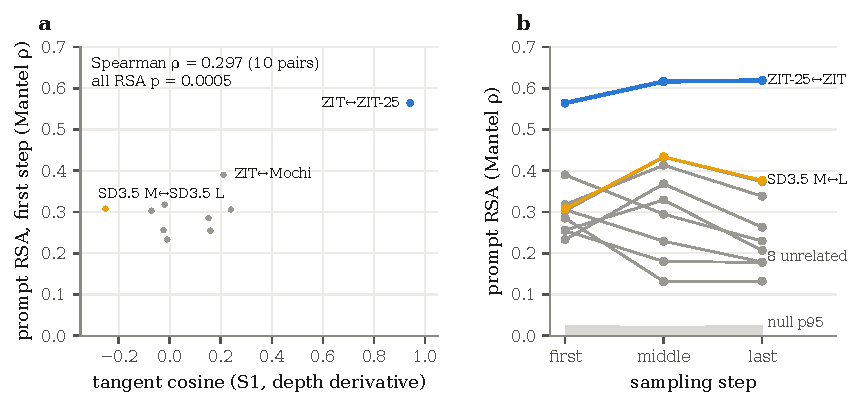
\includegraphics[width=\linewidth]{II-F7_content_vs_dynamics}
 \caption{\textbf{Content geometry and dynamics are different quotients.} (a) For each of the 10 model pairs, the first-step prompt RSA is plotted against the tangent cosine. The RSA is a Mantel $\rho$ between $117\times117$ prompt-distance matrices, with $p=0.0005$ for every pair against its own prompt-permutation null. The rank coupling is weak (Spearman $\rho=0.297$, preregistered S2g). (b) RSA at the first, middle and last step. Unrelated pairs score 0.13--0.43 and \TT{}$\leftrightarrow$ZIT (same weights) 0.56--0.62. Every value lies far above its permutation-null p95 ($\approx0.02$, shaded). Shared content organization exists across unrelated architectures, beyond themes and prompt text (P2), and without a shared microscopic flow. The two are distinct equivalence relations. Sources: \texttt{review/round6/out/S2\_rsa.csv}, \texttt{S1\_hierarchy.csv}; register \#19, T3.}
 \label{fig:content}
\end{figure}

\begin{figure}[p]
 \centering
 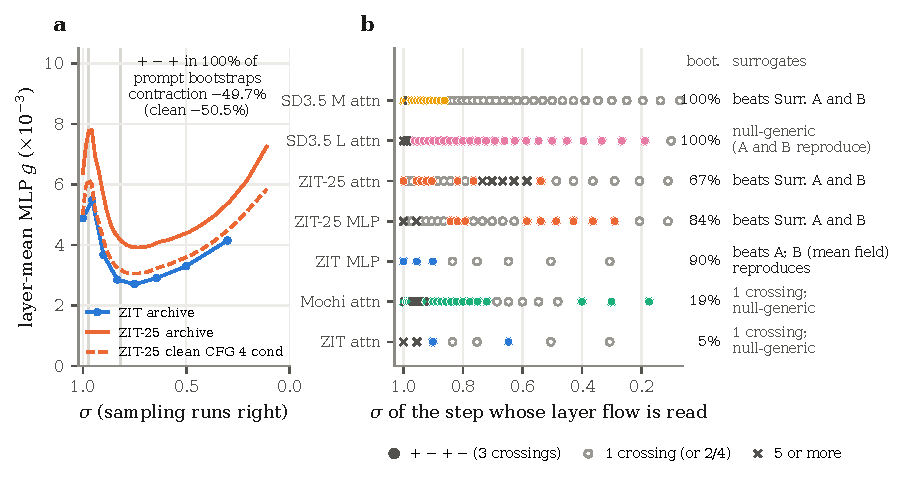
\includegraphics[width=\linewidth]{II-F8_two_axis_topology}
 \caption{\textbf{Two different phase constructions; do not conflate them.} (a) Sampling-clock axis, Z-Image MLP only. Population-mean, layer-mean MLP $g(\sigma)$ is shown for ZIT (8 steps), \TT{} (archive, pooled CFG 4) and the clean \TT{} CFG 4 cond branch, recomputed from the raw cubes. All three are Z-Image Turbo (the 25-step archive files are labelled ZIB); the real Base MLP gives $+++$ (Round 11, not drawn). The three-segment fit gives $+-+$ in 100\% of 1000 prompt bootstraps in every arm (S4a--b). The contraction is $-49.7\%$ in the archive and $-50.5\%$ on the clean branch. Vertical lines mark the \TT{} archive breakpoints, $\sigma=0.972$ and $0.818$. Attention follows a different curve ($++-$) in all five archive channels (S4e, P1), so the $\sigma$-axis result is scoped to Z-Image Turbo MLP. (b) Layer axis, post hoc (analyzer replay A2--A4). The sign pattern of $\beta_{\rm layer}(g)$, binned against $g$, is shown at each sampling step. Right-hand columns give the whole-run generation-bootstrap rate of $+-+-$ and the surrogate class: SD3.5 M attention: 100\%, beats Surrogates A and B; SD3.5 L attention: 100\%, \textbf{null-generic} (per-layer marginals alone reproduce it); \TT{} attention: 67\%, beats A and B; \TT{} MLP: 84\%, beats A and B; ZIT MLP: 90\%, beats A, but B (the mean field $g(L,\sigma)$) reproduces it; Mochi and ZIT attention: a single, null-generic crossing. Not drawn: the real Z-Image Base conditional branch and both ACE-Step checkpoints give one crossing (Rounds 12 and 14; Mode-I Fig.~14). Report the layer-axis pattern per $\sigma$ or with its bootstrap rate and surrogate class, never as one crossing count. Neither panel defines a phase boundary or a separatrix. Sources: \texttt{review/round6/out/S4\_topology.csv}, \texttt{A2\_beta\_layer\_bootstrap.csv}, \texttt{A4\_beta\_layer\_per\_step.csv}, \texttt{A4\_beta\_layer\_surrogates.csv}; raw cubes for the curves in (a); register \#1.}
 \label{fig:topology}
\end{figure}

\begin{figure}[h]
 \centering
 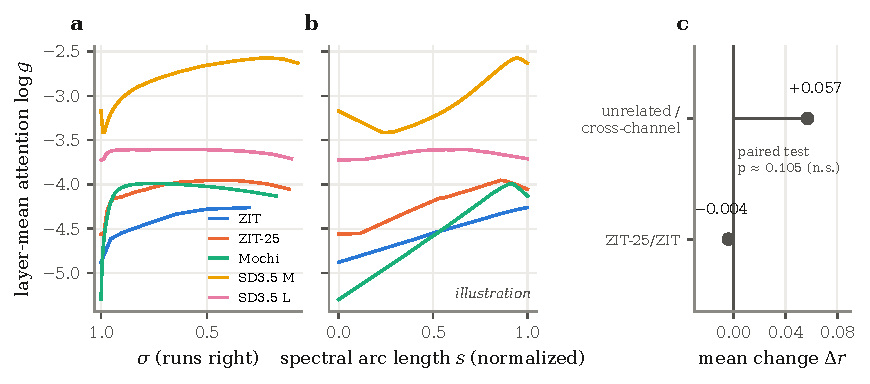
\includegraphics[width=\linewidth]{II-S1_intrinsic_progress}
 \caption{\textbf{Intrinsic progress gives no decisive universal quotient (negative result).} (a,b) Illustration on data: layer-mean attention $\log g$ for the five archive models, plotted against $\sigma$ (a) and against normalized cumulative spectral arc length (b). Here arc length is re-implemented as the path length of the z-scored layer-mean $(\log g,\log{\rm gap},H)$. It shows the reparameterization only and is not the D17 computation. (c) Ledger D17: arc-length reparameterization raises unrelated and cross-channel envelope correlation by $+0.057$ on average. The preregistered paired test is not significant ($p\approx0.105$). \TT{}/ZIT (same weights) changes by $-0.004$. A universal intrinsic-progress quotient is therefore not established.}
 \label{fig:S1}
\end{figure}

\begin{figure}[h]
 \centering
 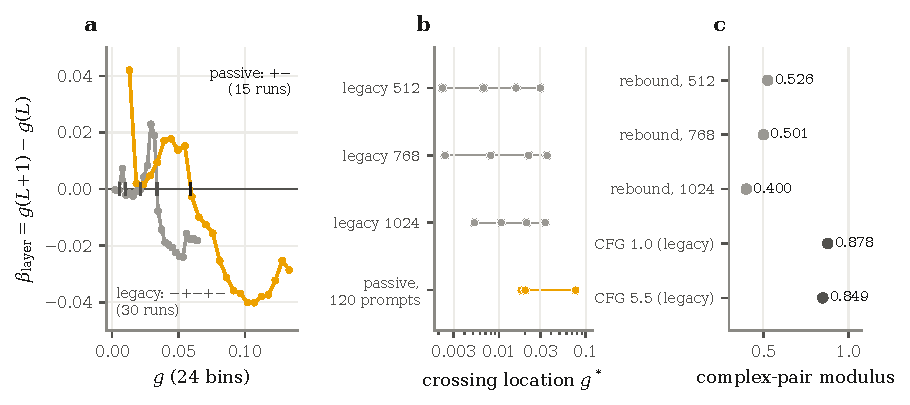
\includegraphics[width=\linewidth]{II-S2_legacy_rebound}
 \caption{\textbf{Legacy rebound and local complex mode: historical, instrument-labelled.} Everything marked \emph{legacy} comes from EMAG-schema files written by an older EMAG-guider build, whose measuring hook substitutes the stale EMA attention. It is shown as the history of the mathematical exploration and is not release evidence. (a) 24-bin $\beta_{\rm layer}(g)$ for a matched 100-step SD3.5 M study with the same prompt and schedule. The 30 legacy-schema runs give $-+-+-$ (four crossings); the 15 current passive runs give $+-$ (one crossing, $g^*=0.059$). Legacy $g$ sits about $10\times$ below passive $g$. The ledger reports the four-crossing pattern for 30/30 single legacy generations and 0/60 single passive prompts. (b) Crossing locations on the legacy resolution suite (512, 768 and 1024 px, single prompt; four crossings each) and on the passive 120-prompt SD3.5 M campaign (three crossings, $g^*=0.018/0.020/0.077$). (c) Complex-pair modulus of the local affine map: on the legacy rebound branch: 0.526, 0.501 and 0.400; in the legacy CFG $1.0\to5.5$ study, steps 0--9: 0.878 [0.862, 0.891] $\to$ 0.849 [0.836, 0.861]. Over all 100 steps of that study, CFG 1.0 has no complex pair. Sources: \texttt{review/round5/reviewer\_v016/results/B7\_MATCHED100\_*}; ledger rebound cards with their v0.12--v0.15 annotations.}
 \label{fig:S2}
\end{figure}
